% Created 2012-06-04 Mon 16:44
\documentclass[11pt]{article}
\usepackage[utf8]{inputenc}
\usepackage[T1]{fontenc}
\usepackage{fixltx2e}
\usepackage{graphicx}
\usepackage{longtable}
\usepackage{float}
\usepackage{wrapfig}
\usepackage{soul}
\usepackage{textcomp}
\usepackage{marvosym}
\usepackage{wasysym}
\usepackage{latexsym}
\usepackage{amssymb}
\usepackage{hyperref}
\tolerance=1000
\providecommand{\alert}[1]{\textbf{#1}}

\title{Rcpp}
\author{Michael Hannon}
\date{\today}
\hypersetup{
  pdfkeywords={},
  pdfsubject={},
  pdfcreator={Emacs Org-mode version 7.8.09}}

\begin{document}

\maketitle

\setcounter{tocdepth}{3}
\tableofcontents
\vspace*{1cm}
\section{A few words about C++}
\label{sec-1}


\begin{itemize}
\item C++ is a statically typed, free-form, multi-paradigm, compiled,
  general-purpose programming language (Wikipedia).
\item Developed by Bjarne Stroustrup at Bell Labs, starting in late 1970's
  as a sort of generalization of the C language (hence, the name).
\item C++ today is a ``federation of four languages'' (Eddelbuettel).
\begin{itemize}
\item Compiled rather than interpreted (like C, Fortran, etc.)
\item OOP (``marries data with code'')
\item Generic programming (Standard Template Library)
\item Template programming
\end{itemize}
\item Many recent developments:
  \href{http://herbsutter.com/2012/04/12/talk-online-not-your-fathers-c-panel/}{http://herbsutter.com/2012/04/12/talk-online-not-your-fathers-c-panel/}
\item Compiled language: like having an instructor peering over your
  shoulder!
\end{itemize}
\section{A few words about Rcpp}
\label{sec-2}
\subsection{Introduction by the primary author}
\label{sec-2-1}


    \href{http://dirk.eddelbuettel.com/code/rcpp.html}{http://dirk.eddelbuettel.com/code/rcpp.html}

In brief:

\begin{quote}

The Rcpp package provides C++ classes that greatly facilitate
interfacing C or C++ code in R packages using the .Call() interface
provided by R. 

\end{quote}

Most of this presentation consists of examples from class notes from a
class given by Dirk Eddelbuetel and Romain Francois.
\subsection{Caveat}
\label{sec-2-2}


Rcpp is a moving target, and much of the documentation that is ``in the
wild'' does \textbf{not} represent the current state of the software.
\subsection{Why use Rcpp?}
\label{sec-2-3}


\begin{itemize}
\item It is often faster than native R
\item It expands the scope of libraries and tools available to R
\end{itemize}
\section{Some examples}
\label{sec-3}
\subsection{A first example: speed}
\label{sec-3-1}



\begin{verbatim}

## cf http://dirk.eddelbuettel.com/blog/2010/09/07#straight_curly_or_compiled

## Xian's code, using <- for assignments and passing x down
f <- function(n, x=1) for (i in 1:n) x=1/(1+x)
g <- function(n, x=1) for (i in 1:n) x=(1/(1+x))
h <- function(n, x=1) for (i in 1:n) x=(1+x)^(-1)
j <- function(n, x=1) for (i in 1:n) x={1/{1+x}}
k <- function(n, x=1) for (i in 1:n) x=1/{1+x}

## R 2.13.0 brings this toy
library(compiler)
lf <- cmpfun(f)
lg <- cmpfun(g)
lh <- cmpfun(h)
lj <- cmpfun(j)
lk <- cmpfun(k)

## now load some tools
library(rbenchmark)

N <- 1e6

## now with Rcpp and C++
library(inline)

## and define our version in C++
src <- 'int n = as<int>(ns);
        double x = as<double>(xs);
        for (int i=0; i<n; i++) x=1/(1+x);
        return wrap(x); '
l <- cxxfunction(signature(ns="integer",
                           xs="numeric"),
                 body=src, plugin="Rcpp")

## now run the benchmark
print(benchmark(f(N,1), g(N,1), h(N,1), j(N,1), k(N,1),
          l(N,1),
          lf(N,1), lg(N,1), lh(N,1), lj(N,1), lk(N,1),
          columns=c("test", "replications",
          "elapsed", "relative"),
          order="relative", replications=10))
\end{verbatim}


\begin{verbatim}
       test replications elapsed  relative
6   l(N, 1)           10   0.118   1.00000
11 lk(N, 1)           10   3.173  26.88983
10 lj(N, 1)           10   3.196  27.08475
7  lf(N, 1)           10   3.218  27.27119
8  lg(N, 1)           10   3.335  28.26271
9  lh(N, 1)           10   4.326  36.66102
1   f(N, 1)           10  14.633 124.00847
5   k(N, 1)           10  14.693 124.51695
4   j(N, 1)           10  16.256 137.76271
2   g(N, 1)           10  16.706 141.57627
3   h(N, 1)           10  21.476 182.00000
\end{verbatim}
\subsection{RInside: the other way around}
\label{sec-3-2}


Rcpp includes a related R package, \emph{RInside}, which makes it possible
to embed R in C++ applications.
\subsubsection{RInside: the ``hello world'' example}
\label{sec-3-2-1}


It's complicated to include the appropriate libraries, but RInside
comes with a helpful Makefile.  On my system it is located in:


\begin{verbatim}
/usr/lib64/R/library/RInside/examples/standard/Makefile
\end{verbatim}

We want to ``tangle'' the following source-code block, but we need to
preserve the leading tab characters in order to keep ``make'' happy:


\begin{verbatim}

(setq org-src-preserve-indentation t)
\end{verbatim}

Here's the Makefile:


\begin{verbatim}

## -*- mode: make; tab-width: 8; -*-
##
## Simple Makefile
##
## TODO: 
##  proper configure for non-Debian file locations,   [ Done ]
##  allow RHOME to be set for non-default R etc

## comment this out if you need a different version of R, 
## and set set R_HOME accordingly as an environment variable

R_HOME :=               $(shell R RHOME)

sources :=              $(wildcard *.cpp)
programs :=             $(sources:.cpp=)


## include headers and libraries for R 
RCPPFLAGS :=            $(shell $(R_HOME)/bin/R CMD config --cppflags)
RLDFLAGS :=             $(shell $(R_HOME)/bin/R CMD config --ldflags)
RBLAS :=                $(shell $(R_HOME)/bin/R CMD config BLAS_LIBS)
RLAPACK :=              $(shell $(R_HOME)/bin/R CMD config LAPACK_LIBS)

## if you need to set an rpath to R itself, also uncomment
#RRPATH :=              -Wl,-rpath,$(R_HOME)/lib

## include headers and libraries for Rcpp interface classes
RCPPINCL :=             $(shell echo 'Rcpp:::CxxFlags()' | $(R_HOME)/bin/R --vanilla --slave)
RCPPLIBS :=             $(shell echo 'Rcpp:::LdFlags()'  | $(R_HOME)/bin/R --vanilla --slave)


## include headers and libraries for RInside embedding classes
RINSIDEINCL :=          $(shell echo 'RInside:::CxxFlags()' | $(R_HOME)/bin/R --vanilla --slave)
RINSIDELIBS :=          $(shell echo 'RInside:::LdFlags()'  | $(R_HOME)/bin/R --vanilla --slave)

## compiler etc settings used in default make rules
CXX :=                  $(shell $(R_HOME)/bin/R CMD config CXX)
CPPFLAGS :=             -Wall $(shell $(R_HOME)/bin/R CMD config CPPFLAGS)
CXXFLAGS :=             $(RCPPFLAGS) $(RCPPINCL) $(RINSIDEINCL) $(shell $(R_HOME)/bin/R CMD config CXXFLAGS)
LDLIBS :=               $(RLDFLAGS) $(RRPATH) $(RBLAS) $(RLAPACK) $(RCPPLIBS) $(RINSIDELIBS)

all:                    $(programs)
                        @test -x /usr/bin/strip && strip $^

run:                    $(programs)
                        @for p in $(programs); do echo; echo "Running $$p:"; ./$$p; done

clean:
                        rm -vf $(programs)
                        rm -vrf *.dSYM

runAll:
                        for p in $(programs); do echo "Running $$p"; ./$$p; done
\end{verbatim}


Here's the C++ code for the ``hello world'' program:


\begin{verbatim}

#include <RInside.h>              // embedded R via RInside

int main(int argc, char *argv[]) {

    RInside R(argc, argv);        // create embedded R inst.

    R["txt"] = "Hello, world!\n"; // assign  to 'txt' in R

    R.parseEvalQ("cat(txt)");     // eval string, ignore result

    exit(0);
}
\end{verbatim}


\begin{verbatim}

make -f Makefile.demo
./RI-hw
\end{verbatim}
\subsubsection{RInside: use of R graphics in C++}
\label{sec-3-2-2}






\begin{verbatim}
 Starting R at:
 [1] "2012-06-04 16:46:09 PDT"
 Could now use plot in RIgraphics.png
\end{verbatim}


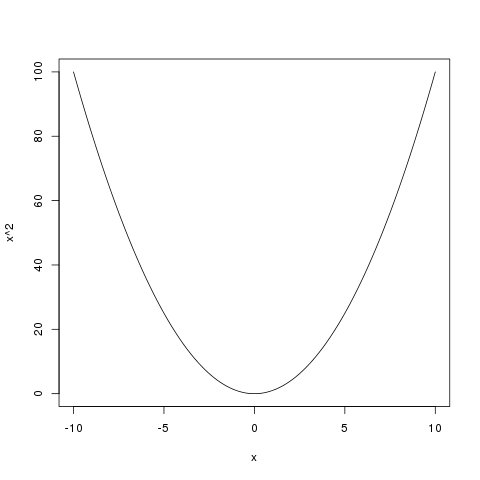
\includegraphics[width=.9\linewidth]{./RIgraphics.png}
\subsection{Product of integer vector with C++ loop}
\label{sec-3-3}



\begin{verbatim}

library(inline)

src <- '
    Rcpp::IntegerVector vec(vx);
    int prod = 1;
    for (int i=0; i<vec.size(); i++) {
        prod *= vec[i];
    }
    return Rcpp::wrap(prod);
'
funLoop <- cxxfunction(signature(vx="integer"),
                   src, plugin="Rcpp")
funLoop(1L:10L)


## Can also use a sort of "vectorized" approach

src <- '
  Rcpp::IntegerVector vec(vx);
  int prod = std::accumulate(vec.begin(), vec.end(),
                             1, std::multiplies<int>());
  return Rcpp::wrap(prod);
'
funVec <- cxxfunction(signature(vx="integer"),
                   src, plugin="Rcpp")
funVec(1L:10L)


## But there's not much (or any) performance advantage
###### This needs work ###################################

library(rbenchmark)

print(benchmark(funLoop(1L:1000L), funVec(1L:1000L),
          columns=c("test",    "replications",
                    "elapsed", "relative"),
          order=c("replications", "elapsed"), replications=10^(1:5)))
\end{verbatim}


\begin{verbatim}
[1] 3628800
[1] 3628800
              test replications elapsed relative
1  funLoop(1:1000)           10   0.000        0
6   funVec(1:1000)           10   0.000        0
2  funLoop(1:1000)          100   0.001        1
7   funVec(1:1000)          100   0.001        1
8   funVec(1:1000)         1000   0.010       10
3  funLoop(1:1000)         1000   0.014       14
9   funVec(1:1000)        10000   0.109      109
4  funLoop(1:1000)        10000   0.153      153
10  funVec(1:1000)       100000   1.104     1104
5  funLoop(1:1000)       100000   1.598     1598
\end{verbatim}
\section{A peek under the hood}
\label{sec-4}


\begin{quote}

The RObject class is the basic class behind the new API.

It is a thin wrapper around a SEXP object.  This is often called a
proxy model as we do not copy the R object.

RObject manages the life cycle, the object is protected from
garbage collection while in scope -- so you do not have to do
memory management.

-- Dirk Eddelbuettel


\end{quote}
\section{Some words about constructors}
\label{sec-5}
\subsection{Nasty example: ``remember to clone''}
\label{sec-5-1}


What is the difference between the two invocations of ``fun'' below?


\begin{verbatim}

library(inline)

src <- '
  NumericVector x1(xs); ////////////////////////////////
  NumericVector x2(Rcpp::clone(xs));
  IntegerVector x3(Rcpp::clone(xs));
  IntegerVector x4(xs); ////////////////////////////////
  x1[0] = 22;
  x2[1] = 44;
  x3[2] = 66;
  x4[0] = 88;
  return(DataFrame::create(Named("orig", xs),
                           Named("x1", x1),
                           Named("x2", x2),
                           Named("x3", x3),
                           Named("x4", x4)));'
fun <- cxxfunction(signature(xs="numeric"),
                   body=src, plugin="Rcpp")
fun(seq(1.0, 3.0, by=1.0))
fun(1L:3L)
\end{verbatim}

\begin{verbatim}
   orig x1 x2 x3 x4
 1   22 22  1  1 88
 2    2  2 44  2  2
 3    3  3  3 66  3
   orig x1 x2 x3 x4
 1   88 22  1  1 88
 2    2  2 44  2  2
 3    3  3  3 66  3
\end{verbatim}

In the first case, R is invoking ``fun'' with a vector of three real
numbers.  Therefore:

\begin{itemize}
\item x1 is type-compatible with the input, xs, and \textbf{no} new vector is
    created
\item x2 and x3 are explicitly cloned, so new vectors \textbf{are} created for
    both
\item x4 is \textbf{not} type-compatible with the input, so a new vector is
    created
\end{itemize}


Hence, x1 is identical with xs, and when x1 gets changed (\texttt{x1[0] = 22}), so does xs (aka ``orig'').

In the second case, R is invoking ``fun'' with a vector of three
integers.  Therefore:

\begin{itemize}
\item x1 is not type-compatible with the input, so a new vector is
    created
\item x2 and x3 are cloned, as before, so both are new vectors
\item x4 now \textbf{is} type-compatible with the input, so no new vector is
    created for it
\end{itemize}

Hence, x4 is now identical with xs, and when x4 gets changed (\texttt{x4[0] = 88}), so does xs (aka ``orig'')
\subsection{Constructor overview}
\label{sec-5-2}


SEXP x;
NumericVector y( x ); // from a SEXP

// cloning (deep copy)
NumericVector z = clone<NumericVector>( y );

// of a given size (all elements set to 0.0)
NumericVector y( 10 );

// \ldots{} specifying the value
NumericVector y( 10, 2.0 );

// \ldots{} with elements generated
NumericVector y( 10, ::Rf$_{\mathrm{unif}}$$_{\mathrm{rand}}$ );

// with given elements
NumericVector y = NumericVector::create( 1.0, 2.0 );
\section{Matrices}
\label{sec-6}


Matrices are vectors with a dimension attribute.
\subsection{Simple matrix example}
\label{sec-6-1}


Note the use of an ``apply-like'' C++ function here.


\begin{verbatim}

library(inline)

src <- '
  Rcpp::NumericMatrix mat = Rcpp::NumericMatrix(mx);
  std::transform(mat.begin(), mat.end(),
                 mat.begin(), ::sqrt);
  return mat; '
fun <- cxxfunction(signature(mx="numeric"), src,
                   plugin="Rcpp")
mat <- matrix(c(1, 4, 9, 16, 25, 36, 49, 64, 81), 3, 3)
fun(mat)
\end{verbatim}

\begin{verbatim}
      [,1] [,2] [,3]
 [1,]    1    4    7
 [2,]    2    5    8
 [3,]    3    6    9
\end{verbatim}
\subsection{RcppArmadillo}
\label{sec-6-2}


``Armadillo'' is an open-source linear-algebra library for C++:

    \href{http://arma.sourceforge.net/}{http://arma.sourceforge.net/}

The RcppArmadillo package makes it easy to use Armadillo in Rcpp.


\begin{verbatim}

library(inline)

src <- '
  arma::mat m1 = Rcpp::as<arma::mat>(mx);
  arma::mat m2 = m1 + m1;
  arma::mat m3 = m1 * 3;
  return Rcpp::List::create(m1, m2, m3); '
fun <- cxxfunction(signature(mx="numeric"), src,
                   plugin="RcppArmadillo")
mat <- matrix(1:9, 3, 3)
mat2 <- fun(mat)
print(mat2)
\end{verbatim}


\begin{verbatim}
[[1]]
     [,1] [,2] [,3]
[1,]    1    4    7
[2,]    2    5    8
[3,]    3    6    9

[[2]]
     [,1] [,2] [,3]
[1,]    2    8   14
[2,]    4   10   16
[3,]    6   12   18

[[3]]
     [,1] [,2] [,3]
[1,]    3   12   21
[2,]    6   15   24
[3,]    9   18   27
\end{verbatim}


Note, by the way, that some people prefer the ``Eigen'' package for this
kind of thing:


\begin{verbatim}

                Information on package ‘RcppEigen’

Description:

Package:            RcppEigen
Type:               Package
Title:              Rcpp integration for the Eigen templated linear
                    algebra library.
\end{verbatim}
\subsection{More fun with Armadillo: eigenvalues}
\label{sec-6-3}




\begin{verbatim}

library(inline)

src <- '
  arma::mat m1 = Rcpp::as<arma::mat>(mx);
  arma::vec eigval;
  arma::mat eigvec;

  eig_sym(eigval, eigvec, m1);

  return Rcpp::List::create(m1, eigval, eigvec); '
fun <- cxxfunction(signature(mx="numeric"), src,
                   plugin="RcppArmadillo")


mat <- matrix (rbind(c(3, 2, 4),
                     c(2, 0, 2),
                     c(4, 2, 3)), nrow=3, ncol=3)

print(fun(mat))
\end{verbatim}


\begin{verbatim}
[[1]]
     [,1] [,2] [,3]
[1,]    3    2    4
[2,]    2    0    2
[3,]    4    2    3

[[2]]
     [,1]
[1,]   -1
[2,]   -1
[3,]    8

[[3]]
           [,1]       [,2]      [,3]
[1,] -0.4941014 -0.5580496 0.6666667
[2,] -0.4720189  0.8161415 0.3333333
[3,]  0.7301109  0.1499788 0.6666667
\end{verbatim}
\section{Many other data types in Rcpp}
\label{sec-7}
\subsection{GenericVector (List)}
\label{sec-7-1}


We had an example above, in the discussion of eigenvalues.
\subsection{DataFrame}
\label{sec-7-2}


We had an example above in the discussion of cloning.
\subsection{Function}
\label{sec-7-3}
\subsubsection{Example: grabbing a function from R}
\label{sec-7-3-1}


This example merely illustrates the use of Rcpp to link to a function
in R.  All we do is grab the function, apply it to some vectors
created in C++, and then return the output of the function to R.  We
would have gotten the same result had we defined the vectors in R and
invoked the same function directly in R.

But in a real use case, we would have proceede to do further
calculations inside the C+ code.


\begin{verbatim}

library(inline)
src <- '
  Rcpp::Function expGrid("expand.grid");
  IntegerVector v1;
  IntegerVector v2;

  v1.push_back(1);
  v1.push_back(3);
  v1.push_back(5);

  v2.push_back(2);
  v2.push_back(4);
  v2.push_back(6);

  return(expGrid(v1, v2));'

  fun <- cxxfunction(signature(),
                     src,
                     plugin="Rcpp")
  print(fun())
\end{verbatim}


\begin{verbatim}
  Var1 Var2
1    1    2
2    3    2
3    5    2
4    1    4
5    3    4
6    5    4
7    1    6
8    3    6
9    5    6
\end{verbatim}
\subsubsection{Example: passing functions from R to C++}
\label{sec-7-3-2}


Note the third invocation of ``fun''.  In the C++ code the function is
named ``sort'', but that name is, in effect, a dummy variable.


\begin{verbatim}

library(inline)

src <- '
  Function sort(x) ;
  return sort( y, Named("decreasing", true));'
fun <- cxxfunction(signature(x="function",
                             y="ANY"),
                    src, plugin="Rcpp", verbose=FALSE)
fun(sort, sample(1:5, 10, TRUE))
fun(sort, sample(LETTERS[1:5], 10, TRUE))
fun(mean, sample(1:100, 10, TRUE))
\end{verbatim}

\begin{verbatim}
  [1] 5 5 5 5 3 3 3 2 2 1
  [1] "E" "D" "D" "D" "C" "C" "B" "B" "A" "A"
 [1] 58.6
\end{verbatim}
\subsection{Environment}
\label{sec-7-4}


The Environment class allows us to access R environments.  It provides
an alternative way of accessing functions from R.


\begin{verbatim}

library(inline)

src <- '
    Rcpp::Environment stats("package:stats");
    Rcpp::Function rnorm = stats["rnorm"];
    return rnorm(10, Rcpp::Named("sd", 100.0));
'

fun <- cxxfunction(signature(),
                   src, plugin="Rcpp")
fun()
\end{verbatim}

\begin{verbatim}
  [1]  106.093676    1.059361   51.519316   31.036035  -75.344858  -36.977641   71.808983
  [8]  -50.170794 -162.731572  -67.195076
\end{verbatim}
\subsection{S4 classes}
\label{sec-7-5}


S4 classes can also be created or altered at the C++ level.  Example
omitted.
\section{Creating a package with Rcpp}
\label{sec-8}


R provides a function, \texttt{package.skeleton()}, to help create R
packages.

Eddelbuettel/Francois have wrapped and extended this function to
\texttt{Rcpp.package.skeleton()} to help create R packages that involve Rcpp.
\subsection{Making the skeleton}
\label{sec-8-1}



\begin{verbatim}

library(Rcpp)
if (!file.exists("./UCDpackage")) {
    Rcpp.package.skeleton( "UCDpackage" )
}
\end{verbatim}


\begin{verbatim}
 Creating directories ...
Creating DESCRIPTION ...
Creating NAMESPACE ...
Creating Read-and-delete-me ...
Saving functions and data ...
Making help files ...
Done.
Further steps are described in './UCDpackage/Read-and-delete-me'.

Adding Rcpp settings
 >> added Depends: Rcpp
 >> added LinkingTo: Rcpp
 >> added useDynLib directive to NAMESPACE
 >> added Makevars file with Rcpp settings
 >> added Makevars.win file with Rcpp settings
 >> added example header file using Rcpp classes
 >> added example src file using Rcpp classes
 >> added example R file calling the C++ example
 >> added Rd file for rcpp_hello_world
\end{verbatim}
\subsection{A look at the file structure of the skeleton package}
\label{sec-8-2}



\begin{verbatim}

tree UCDpackage
\end{verbatim}


\begin{verbatim}
UCDpackage
├── DESCRIPTION
├── man
│   ├── rcpp_hello_world.Rd
│   └── UCDpackage-package.Rd
├── NAMESPACE
├── R
│   └── rcpp_hello_world.R
├── Read-and-delete-me
└── src
    ├── Makevars
    ├── Makevars.win
    ├── rcpp_hello_world.cpp
    ├── rcpp_hello_world.h
    ├── rcpp_hello_world.o
    └── UCDpackage.so

3 directories, 12 files
\end{verbatim}
\subsection{The C++ header file}
\label{sec-8-3}



\begin{verbatim}

cat ./UCDpackage/src/rcpp_hello_world.h
\end{verbatim}


\begin{verbatim}
#ifndef _UCDpackage_RCPP_HELLO_WORLD_H
#define _UCDpackage_RCPP_HELLO_WORLD_H

#include <Rcpp.h>

/*
 * note : RcppExport is an alias to `extern "C"` defined by Rcpp.
 *
 * It gives C calling convention to the rcpp_hello_world function so that 
 * it can be called from .Call in R. Otherwise, the C++ compiler mangles the 
 * name of the function and .Call can't find it.
 *
 * It is only useful to use RcppExport when the function is intended to be called
 * by .Call. See the thread http://thread.gmane.org/gmane.comp.lang.r.rcpp/649/focus=672
 * on Rcpp-devel for a misuse of RcppExport
 */
RcppExport SEXP rcpp_hello_world() ;

#endif
\end{verbatim}
\subsection{The C++ source file}
\label{sec-8-4}



\begin{verbatim}

cat ./UCDpackage/src/rcpp_hello_world.cpp
\end{verbatim}


\begin{verbatim}
#include "rcpp_hello_world.h"

SEXP rcpp_hello_world(){
    using namespace Rcpp ;
    
    CharacterVector x = CharacterVector::create( "foo", "bar" )  ;
    NumericVector y   = NumericVector::create( 0.0, 1.0 ) ;
    List z            = List::create( x, y ) ;
    
    return z ;
}
\end{verbatim}
\subsection{The R file}
\label{sec-8-5}



\begin{verbatim}

cat ./UCDpackage/R/rcpp_hello_world.R
\end{verbatim}

\begin{verbatim}
 
 rcpp_hello_world <- function(){
 	.Call( "rcpp_hello_world", PACKAGE = "UCDpackage" )
 }
 
\end{verbatim}
\subsection{The DESCRIPTION file}
\label{sec-8-6}


Note the last two lines, which declare the dependency of your package
on Rcpp.


\begin{verbatim}

cat ./UCDpackage/DESCRIPTION
\end{verbatim}


\begin{verbatim}
Package: UCDpackage
Type: Package
Title: What the package does (short line)
Version: 1.0
Date: 2012-06-04
Author: Who wrote it
Maintainer: Who to complain to <yourfault@somewhere.net>
Description: More about what it does (maybe more than one line)
License: What Licence is it under ?
Depends: Rcpp (>= 0.9.10)
LinkingTo: Rcpp
\end{verbatim}
\subsection{The NAMESPACE file}
\label{sec-8-7}


The regular expression exports all symbols.


\begin{verbatim}

cat ./UCDpackage/NAMESPACE
\end{verbatim}

\begin{verbatim}
 useDynLib(UCDpackage)
 exportPattern("^[[:alpha:]]+")
\end{verbatim}
\subsection{The standard Makevars file}
\label{sec-8-8}



\begin{verbatim}

cat ./UCDpackage/src/Makevars
\end{verbatim}


\begin{verbatim}
## Use the R_HOME indirection to support installations of multiple R version
PKG_LIBS = `$(R_HOME)/bin/Rscript -e "Rcpp:::LdFlags()"`

## As an alternative, one can also add this code in a file 'configure'
##
##    PKG_LIBS=`${R_HOME}/bin/Rscript -e "Rcpp:::LdFlags()"`
## 
##    sed -e "s|@PKG_LIBS@|${PKG_LIBS}|" \
##        src/Makevars.in > src/Makevars
## 
## which together with the following file 'src/Makevars.in'
##
##    PKG_LIBS = @PKG_LIBS@
##
## can be used to create src/Makevars dynamically. This scheme is more
## powerful and can be expanded to also check for and link with other
## libraries.  It should be complemented by a file 'cleanup'
##
##    rm src/Makevars
##
## which removes the autogenerated file src/Makevars. 
##
## Of course, autoconf can also be used to write configure files. This is
## done by a number of packages, but recommended only for more advanced users
## comfortable with autoconf and its related tools.
\end{verbatim}
\subsection{The Windows Makevars.win file}
\label{sec-8-9}



\begin{verbatim}

cat ./UCDpackage/src/Makevars.win
\end{verbatim}

\begin{verbatim}
 
 ## Use the R_HOME indirection to support installations of multiple R version
 PKG_LIBS = $(shell "${R_HOME}/bin${R_ARCH_BIN}/Rscript.exe" -e "Rcpp:::LdFlags()")
\end{verbatim}
\subsection{Installation}
\label{sec-8-10}


Something in my .Rprofile was causing a problem.


\begin{verbatim}

mv ~/.Rprofile ~/.Rprofile.save
R CMD INSTALL -l ~/R/library UCDpackage
mv ~/.Rprofile.save ~/.Rprofile
\end{verbatim}

\begin{verbatim}
 make: Nothing to be done for `all'.
   converting help for package ‘UCDpackage’
     UCDpackage-package                      html  
     rcpp_hello_world                        html  
\end{verbatim}
\subsection{Use of the package}
\label{sec-8-11}




\begin{verbatim}

library("UCDpackage", lib.loc="~/R/library")
rcpp_hello_world()
\end{verbatim}

\begin{verbatim}
 [[1]]
 [1] "foo" "bar"
 
 [[2]]
 [1] 0 1
\end{verbatim}
\section{Syntactic sugar}
\label{sec-9}


\begin{quote}

Put succinctly, the motivation of Rcpp sugar is to bring a subset of
the high-level R syntax in C++.

-- Dirk Eddelbuettel and Romain Francois

\end{quote}

See the PDF document in the vignette:


\begin{verbatim}

> vignette("Rcpp-sugar")
\end{verbatim}
\subsection{A first sugar example: sapply}
\label{sec-9-1}


To use an auxiliary function with the simple ``inline'' approach, the
function, AFAICT, has to be defined in an include file.

But, given the function, the syntax for sapply in C++  is now virtually
identical to the syntax used in R.  (The ``wrap'' function is a part of
Rcpp that transforms an arbitrary object into a symbolic expression,
aka, SEXP -- i.e. something that R can understand.)


\begin{verbatim}

library(inline)
includes <- '
        double square( double x){
          return x*x ;
        }'

src <- 'NumericVector x(xx);
        return wrap(sapply( x, square ));'

fun <- cxxfunction(signature(xx="numeric"),
                   body=src,
                   plugin="Rcpp",
                   includes=includes)

fun(c(1, 3, 5, 7, 9))
\end{verbatim}

\begin{verbatim}
 [1]  1  9 25 49 81
\end{verbatim}
\subsection{Sugar example with benchmark}
\label{sec-9-2}


Note that the C++ syntax is very ``R-like'', but that there is a
significant performance advantage to using Rcpp/C++.


\begin{verbatim}

foo <- function(x) {

    ## sum of
    ##  -- squares of negatives
    ##  -- exponentials of positives
    s <- sum(ifelse( x < 0,  x*x,  exp(x) ))

    return(s)
}


library(inline)

cppfoo <- cxxfunction(signature(xs="numeric"),
                   plugin="Rcpp", body='

   NumericVector x(xs);

   double s = sum( ifelse( x < 0, x*x, exp(x) ));

   return wrap(s);
')

library(compiler)
Rcmpfoo <- cmpfun(foo)

library(rbenchmark)
x <- rnorm(1e5)
benchmark(foo(x), Rcmpfoo(x), cppfoo(x),
          columns=c("test", "elapsed", "relative", "user.self", "sys.self"),
          order="relative", replications=10)
\end{verbatim}

\begin{verbatim}
         test elapsed relative user.self sys.self
 3  cppfoo(x)   0.035  1.00000     0.035    0.000
 2 Rcmpfoo(x)   0.654 18.68571     0.653    0.000
 1     foo(x)   0.890 25.42857     0.889    0.001
\end{verbatim}

\end{document}
